\documentclass{beamer}

\mode<presentation> {
\usetheme{Madrid}
}

\usepackage{graphicx}
\usepackage{booktabs}
\usepackage{polski}
\usepackage[polish]{babel}
\usepackage[utf8]{inputenc}
\usepackage[T1]{fontenc}
\usepackage[utf8]{luainputenc}
\usepackage{pgfgantt}
\usepackage{caption}
\usepackage{mwe}

% Strona tytułowa
\usepackage{pgfplots}
\usepackage{siunitx}
\usepackage{paracol}
\usepackage{gensymb}

% Pływające obrazki
\usepackage{float}
\usepackage{svg}
\usepackage{graphicx}
\usepackage{subfig}


\sisetup{group-digits=true,
        %  group-four-digits=true,
        round-precision=4,
        group-separator={},
        output-decimal-marker={,}}

\DeclareCaptionFormat{citation}{%
   \ifx\captioncitation\relax\relax\else
     \captioncitation\par
   \fi
   #1#2#3\par}
\newcommand*\setcaptioncitation[1]{\def\captioncitation{\tiny{\textit{Źródło:}~#1}\medskip}\normalsize}
\let\captioncitation\relax
\captionsetup{format=citation,justification=centering}

\usetikzlibrary{pgfplots.groupplots}
\sisetup{detect-weight,exponent-product=\cdot,output-decimal-marker={,},per-mode=symbol,binary-units=true,range-phrase={-},range-units=single}

%wymiar tekstu
\def\figurename{Rys.}
\def\tablename{Tab.}

%----------------------------------------------------------------------------------------
%	TITLE PAGE
%----------------------------------------------------------------------------------------

\title[WEDT - Projekt]{Wprowadzenie do eksploracji danych tekstowych w~sieci~WWW}

\author[Konieczka, Poturała, Sikora]{Maria Konieczka \and Alicja Poturała \and Jakub Sikora} 

\date{3 czerwca 2020}
\institute[]{Odpowiadanie na pytania ogólne zadane w~języku polskim}

\AtBeginSection[]
{
    \begin{frame}[plain, noframenumbering]
        \frametitle{Agenda}
        \tableofcontents[currentsection]
    \end{frame}
}

\begin{document}

\begin{frame}
\titlepage
\end{frame}

\begin{frame}
  \frametitle{Agenda}
  \tableofcontents
\end{frame}

\section{Wprowadzenie w problem}

\begin{frame}
  \frametitle{Definicja zadania}
  \begin{block}{Zadanie odpowiadania na pytania}
    Zadanie odpowiadania na pytania polega na automatycznej \begin{itemize}
      \item analizie otrzymanego pytania w~języku naturalnym,
      \item wyszukiwaniu odpowiednich dokumentów,
      \item ekstrakcji wiedzy,
      \item generacji odpowiedzi, również w~języku naturalnym. 
    \end{itemize}
  \end{block}
\end{frame}

\begin{frame}
  \frametitle{Założenia systemu}
  \begin{block}{Główne założenia systemu:}
  \begin{itemize}
    \item pytania zadawane są w~języku polskim,
    \item system analizuje wiedzę zapisaną w~postaci podsumowań wyników wyszukiwarek internetowych,
    \item system odpowiada na zamknięty zestaw kategorii (domen),
    \item system odpowiada w~postaci jednego do trzech wyrazów, nie zajmujemy się generacją zdań.
  \end{itemize}
\end{block}
\end{frame}

\section{Algorytm wyszukiwania odpowiedzi}
\begin{frame}
  \frametitle{Ogólny opis algorytmu wyszukiwania}
  \bigskip
  \begin{figure}
    \centering
    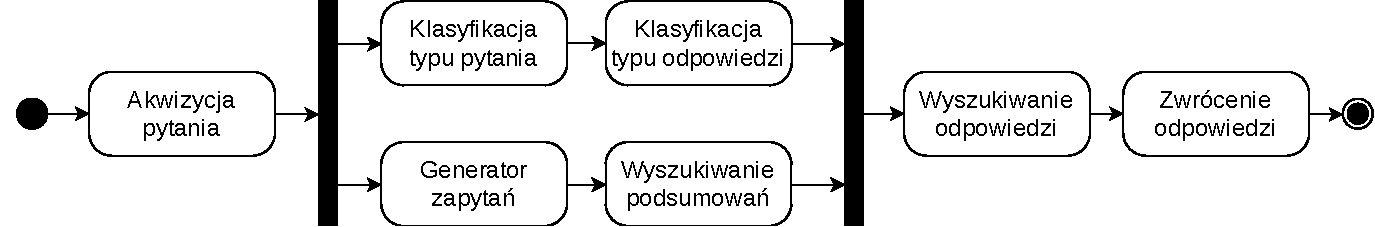
\includegraphics[width=\columnwidth]{figures/WEDT-Algorytm-Rotated.pdf}
    \caption{Ogólny schemat blokowy algorytmu wyszukiwania odpowiedzi}
    \label{fig:ir-algorytm}
  \end{figure}
\end{frame}

\begin{frame}
  \frametitle{Akwizycja pytania}

\end{frame}

\begin{frame}
  \frametitle{Generacja zapytań}

\end{frame}

\begin{frame}
  \frametitle{Wyszukiwanie podsumowań}

\end{frame}

\begin{frame}
  \frametitle{Klasyfikacja typu pytania}

\end{frame}

\begin{frame}
  \frametitle{Klasyfikacja typu odpowiedzi}

\end{frame}

\begin{frame}
  \frametitle{Wyszukiwanie odpowiedzi}

\end{frame}

\begin{frame}
  \frametitle{Zwrócenie odpowiedzi}

\end{frame}

\section{Implementacja i korzystanie z systemu}
\begin{frame}
  \frametitle{Architektura mikroserwisowa}
  \begin{figure}
    \centering
    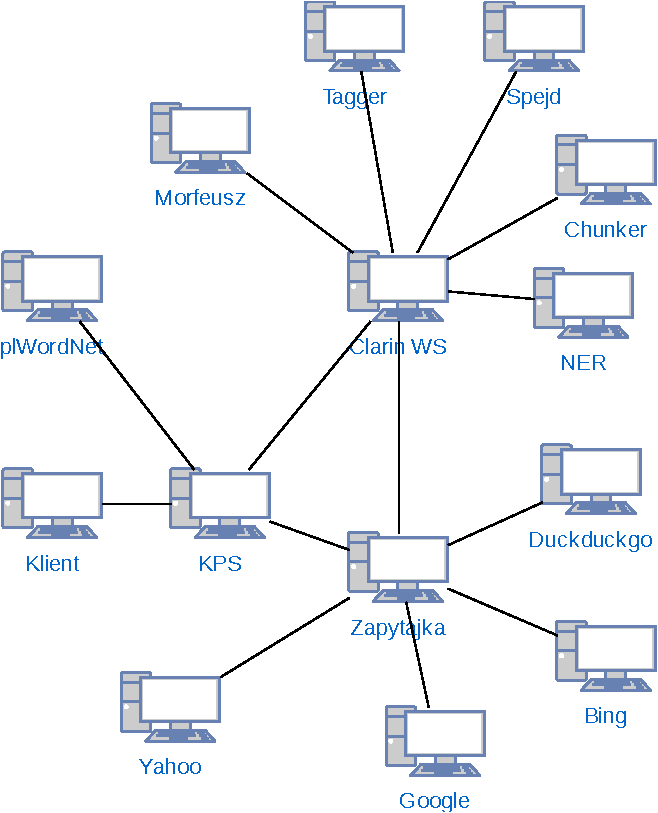
\includegraphics[width=0.5\columnwidth]{figures/WEDT-Uslugi.pdf}
    \label{fig:klient}
  \end{figure}
\end{frame}

\begin{frame}
  \frametitle{Implementacja systemu}
  \begin{block}{Implementacja modułów:}
    \begin{itemize}
      \item odpowiadania na pytania,
      \item klienta internetowego,
      \item \textit{webscrapera} wyszukiwarek internetowych.
    \end{itemize}
  \end{block}

  \begin{block}{Integracja z usługami:}
    \begin{itemize}
      \item plWordNet,
      \item CLARIN WS
      \begin{itemize}
        \item morfeusz,
        \item tagger,
        \item spejd,
        \item chunker,
        \item Named-Entity Recognition.
      \end{itemize}
    \end{itemize}
  \end{block}
\end{frame}

\begin{frame}
  \frametitle{Klient systemu} 
  \begin{figure}
    \centering
    \fbox{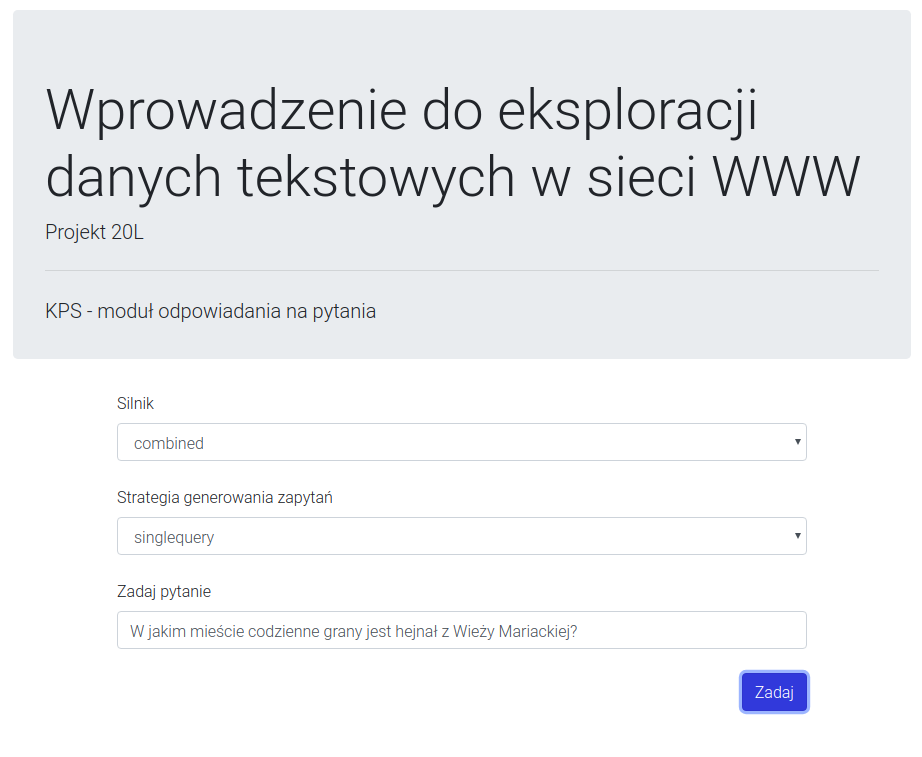
\includegraphics[width=0.7\columnwidth]{figures/kps.png}}
    \label{fig:klient}
  \end{figure}
\end{frame}

\begin{frame}
  \frametitle{Klient systemu} 
  \begin{figure}
    \centering
    \fbox{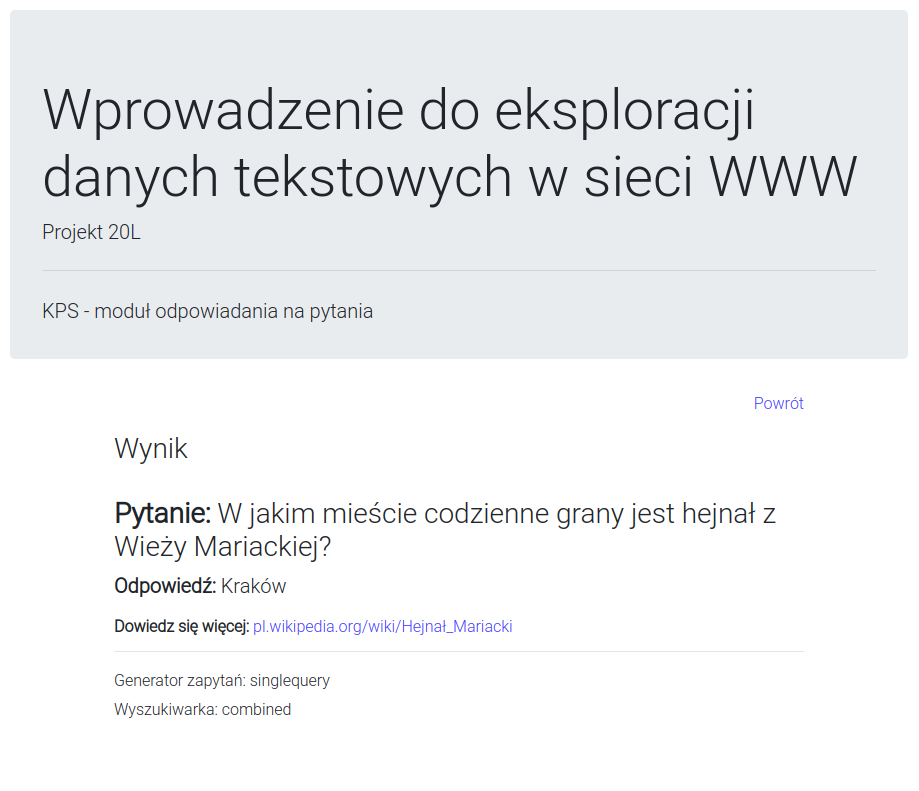
\includegraphics[width=0.7\columnwidth]{figures/kps-answer.png}}
    \label{fig:klient-odp}
  \end{figure}
\end{frame}

\section{Wyniki badań}
\begin{frame}
  \frametitle{Badanie wyszukiwarek internetowych}
  \begin{figure}
    \begin{tikzpicture}
        \begin{axis}[
            grid=both,
            width=\columnwidth,
            height=7.5cm,
            ybar,
            ymin=0,
            bar width=0.5cm,
            enlarge x limits=0.2,
            area legend,
            legend style={at={(0.5,-0.15)},
            anchor=north,
            legend columns=2},
            ylabel={Liczba odpowiedzi},
            symbolic x coords={dobra, częściowo, błędna, brak},
            xtick=data,
            nodes near coords,
            x label style={
            fixed},
            ]
        \legend{google, duckduckgo}
        \addplot coordinates {(dobra,80) (częściowo,8) (błędna,137) (brak,31)};
        \addplot coordinates {(dobra,66) (częściowo,3) (błędna,111) (brak,76)};
		\end{axis}
        \end{tikzpicture}
        \label{fig:porownanie-wyszukiwarek}
  \end{figure}
\end{frame}

\begin{frame}
  \frametitle{Badanie strategii generacji zapytań}

\end{frame}

\section{Wnioski i przemyślenia}
\begin{frame}
  \frametitle{Wnioski z projektu}
  \begin{block}{Wychwytywanie dat}
    Wyrażenia regularne dobrze sprawdzają się przy odpowiadaniu na pytania o~daty.
  \end{block}

  \begin{block}{Pytania jakościowe i ilościowe}
    Przedstawiony algorytm słabo radzi sobie z pytaniami jakościowymi (\textit{jak?}) oraz ilościowymi (\textit{ile?}), z~racji ich ogólnego charakteru.
  \end{block}

  \begin{block}{Półautomatyczne testowanie}
    W~przypadku testowania systemu tego typu, wymagana jest obecność człowieka do jakościowego oceniania wygenerowanych odpowiedzi.
  \end{block}
\end{frame}

\begin{frame}
  \frametitle{Perspektywy rozwoju}
  \begin{block}{Zwiększenie liczby obsługiwanych domen}
    Większa liczba domen pozwoli na odpowiadanie na większą ilość pytań. Docelowo, program może obsługiwać wszystkie domeny z~\textit{plWordNetu}.
  \end{block}

  \begin{block}{Analiza pełnych dokumentów}
    Analiza pełnych dokumentów zamiast podsumowań pozwoliłaby na zwiększenie bazy wiedzy.
  \end{block}

  \begin{block}{Klasyfikacja typów}
    Klasyfikatory oparte o~sieci neuronowe mogłyby pozwolić na zwiększenie dokładności klasyfikacji typu pytania i~odpowiedzi.
  \end{block}

\end{frame}

\begin{frame}
  \frametitle{Podsumowanie}
  W~ramach projektu z~przedmiotu WEDT udało się zrealizować:
  \begin{itemize}
    \item działający system oparty o IR, odpowiadający na pytania w~języku polskim,
    \item moduł integrujący ogólnodostępne narzędzia, wpisujący się w~nowoczesną architekturę opartą o~mikroserwisy,
    \item moduł zbierający dane z~wyszukiwarek internetowych,
    \item szereg eksperymentów testujących podstawowe parametry systemu,
    \item przedstawić możliwości rozwoju przygotowanego systemu.
  \end{itemize}

\end{frame}

\end{document}
